\documentclass[journal]{IEEEtran}
\usepackage[a5paper, margin=10mm, onecolumn]{geometry}
\usepackage{lmodern}
\usepackage{tfrupee}
\setlength{\headheight}{1cm}
\setlength{\headsep}{0mm}

\usepackage{gvv-book}
\usepackage{gvv}
\usepackage{cite}
\usepackage{amsmath,amssymb,amsfonts,amsthm}
\usepackage{algorithmic}
\usepackage{graphicx}
\usepackage{textcomp}
\usepackage{xcolor}
\usepackage{txfonts}
\usepackage{listings}
\usepackage{enumitem}
\usepackage{mathtools}
\usepackage{gensymb}
\usepackage{comment}
\usepackage[breaklinks=true]{hyperref}
\usepackage{tkz-euclide}
\usepackage{listings}
\def\inputGnumericTable{}
\usepackage[latin1]{inputenc}
\usepackage{color}
\usepackage{array}
\usepackage{longtable}
\usepackage{calc}
\usepackage{multirow}
\usepackage{hhline}
\usepackage{ifthen}
\usepackage{lscape}
\usepackage{xparse}

\bibliographystyle{IEEEtran}

\title{4.7.40}
\author{EE25BTECH11043 - Nishid Khandagre} % Replace with your name

\begin{document}
\maketitle

\renewcommand{\thefigure}{\theenumi}
\renewcommand{\thetable}{\theenumi}

\numberwithin{equation}{enumi}
\numberwithin{figure}{enumi}

\textbf{Question}:\
Find the foot of the perpendicular and the perpendicular distance from the point $\myvec{2 \\ 3 \\ -8}$ to the line $\frac{4-x}{2}=\frac{y}{6}=\frac{1-z}{3}$.

\textbf{Solution: }
Given line: 
\begin{align}
\frac{4-x}{2}=\frac{y}{6}=\frac{1-z}{3}=t
\end{align}

\begin{align}
x &= 4-2t \\
y &= 6t \\
z &= 1-3t
\end{align}

Line in vector form:
\begin{align}
\myvec{x \\ y \\ z} = \myvec{4 \\ 0 \\ 1} + t \myvec{-2 \\ 6 \\ -3}
\end{align}
\begin{align}
\vec{r} &= \vec{a} + t \vec{m} \\
\vec{a} &= \myvec{4 \\ 0 \\ 1} \\
\vec{m} &= \myvec{-2 \\ 6 \\ -3}
\end{align}
Given point: $\vec{p} = \myvec{2 \\ 3 \\ -8}$.\\ \\


Let the foot of the perpendicular be $\vec{f}$. Since $\vec{f}$ lies on the line, we can write:
\begin{align}
\vec{f} &= \vec{a} + \alpha\vec{m}
\end{align}


$\myvec{\vec{p} - \vec{f}}$ must be orthogonal to the direction vector of the line $\vec{m}$.\\ \\
Therefore
\begin{align}
\myvec{\vec{p} - \vec{f}}^\top \vec{m} = 0\\
\myvec{\vec{p} - \myvec{\vec{a} + \alpha\vec{m}}}^\top \vec{m} = 0\\
\myvec{\vec{p} - \vec{a} - \alpha\vec{m}}^\top \vec{m} = 0\\
\myvec{\vec{p} - \vec{a}}^\top \vec{m} - \alpha \myvec{\vec{m}^\top \vec{m}} = 0
\end{align}

\begin{align}
\alpha &= \frac{\myvec{\vec{p}-\vec{a}}^\top \vec{m}}{\vec{m}^\top \vec{m}}
\end{align}
\begin{align}
\vec{p}-\vec{a} &= \myvec{2 \\ 3 \\ -8} - \myvec{4 \\ 0 \\ 1} = \myvec{-2 \\ 3 \\ -9}
\end{align}
\begin{align}
\myvec{\vec{p}-\vec{a}}^\top \vec{m} &= \myvec{-2 & 3 & -9} \myvec{-2 \\ 6 \\ -3} \\
&= (-2)(-2) + (3)(6) + (-9)(-3) \\
&= 4 + 18 + 27 = 49
\end{align}
\begin{align}
\vec{m}^\top \vec{m} &= (-2)^2 + 6^2 + (-3)^2 \\
&= 4 + 36 + 9 = 49
\end{align}
Therefore
\begin{align}
\alpha &= \frac{49}{49} = 1
\end{align}
foot of the perpendicular $\vec{f}$:
\begin{align}
\vec{f} &= \vec{a} + \alpha\vec{m} \\
&= \myvec{4 \\ 0 \\ 1} + 1 \myvec{-2 \\ 6 \\ -3} \\
&= \myvec{2 \\ 6 \\ -2}
\end{align}

\begin{align}
\text{Perpendicular Distance} &= \norm{\vec{p}-\vec{f}}
\end{align}
\begin{align}
\vec{p}-\vec{f} &= \myvec{2 \\ 3 \\ -8} - \myvec{2 \\ 6 \\ -2} \\
&=\myvec{0 \\ -3 \\ -6}
\end{align}
\begin{align}
\norm{\vec{p}-\vec{f}} &= \sqrt{\myvec{\vec{p}-\vec{f}}^\top \myvec{\vec{p}-\vec{f}}} \\
&= \sqrt{0^2 + (-3)^2 + (-6)^2} \\
&= \sqrt{0 + 9 + 36} \\
&= \sqrt{45} \\
&= 3\sqrt{5}
\end{align}
The perpendicular distance is $3\sqrt{5}$.
\begin{figure}[H]
\centering
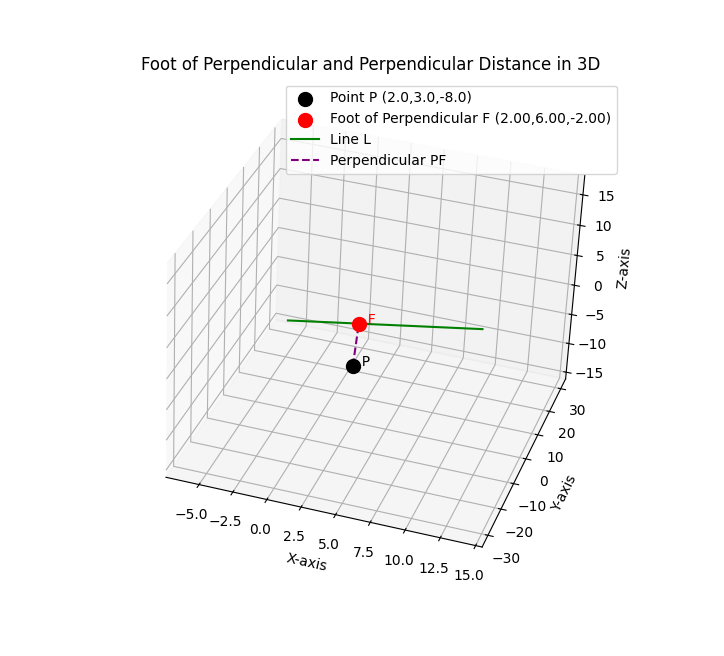
\includegraphics[width=0.8\columnwidth]{figs/fig2.png}
\caption{}
\label{fig:1}
\end{figure}
\end{document}
